\noindent

\includegraphics[height=1.25cm]{images/pictograms/replication}
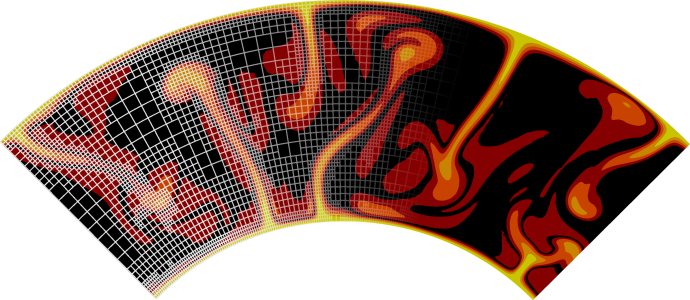
\includegraphics[height=1.25cm]{images/pictograms/aspect_logo}

\includegraphics[height=1.25cm]{images/pictograms/benchmark}

\includegraphics[height=1.25cm]{images/pictograms/FEM}
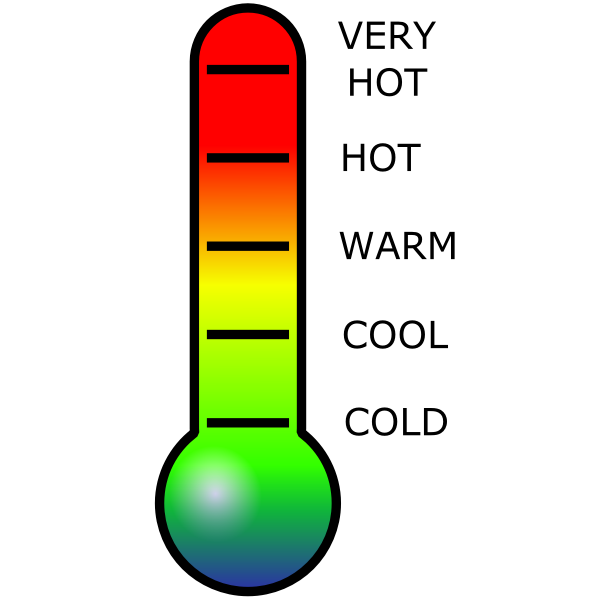
\includegraphics[height=1.25cm]{images/pictograms/temperature}

\includegraphics[height=1.25cm]{images/pictograms/paraview}

%%%%%%%%%%%%%%%%%%%%%%%%%%%%%%%%%%%%%%%%%%%%%%%%%%%%%%%%%%%%%%%%%%%%%%%%%%%%%%%%%%%%%%%%%%%%%%%%%%%

%\lstinputlisting[language=bash,basicstyle=\small]{python_codes/fieldstone_43/keywords.ascii}

\begin{center}
Code at \url{https://github.com/cedrict/fieldstone/tree/master/python_codes/fieldstone_43}
\end{center}

\par\noindent\rule{\textwidth}{0.4pt}

Last revision: Jan. 17th, 2025.

\par\noindent\rule{\textwidth}{0.4pt}

%%%%%%%%%%%%%%%%%%%%%%%%%%%%%%%%%%%%%%%%%%%%%%%%%%%%%%%%%%%%%%%%%%%%%%%%%%%%%%%%%%%%%%%%%%%%

The following experiments are ``pure advection'' experiments (i.e. there is 
no diffusion at all). As such the Peclet number
is infinite and the $\gamma$ value of the SUPG algorithm as shown in Section~\ref{MMM-ss:supg} tends to 1
and the $\tau$ parameter is simply $h/2 |\vec\upnu| p$ (where $p$ is the order of 
the shape function polynomials).

Note that although the code can deal with linear elements, all results 
hereafter are obtained with quadratic elements (unless specified otherwise). 

A very important remark: In step-9 of deal.II (which is concerned with solving the 
steady-state advection equation) we read: `` The mathematical theory states that we must not 
pose any boundary condition on the outflow part of the boundary.''
Upon my asking for more context to Wolfgang Bangerth (the author of step-9), his answer was:
``I think the statement can be shown in the following way: If
you think of the advection equation as transporting information along
characteristics, then the interior can only be affected by characteristics
that go from the boundary into the interior. That's exactly the ones at inflow
boundary conditions. ''
Note that \aspect automatically checks that $\vec\upnu\cdot\vec{n}<0$ at each node where temperature is
prescribed and only prescribe it there
\footnote{\url{https://github.com/geodynamics/aspect/blob/main/source/simulator/core.cc}, Lines 689-726} 
In other words, one cannot prescribe the temperature on a
boundary where the fluid is leaving the domain, only where it is entering.

\todo[inline]{This means that in the experiments presented hereafter this
needs to be checked and corrected if needed!}




\newpage
%------------------------------------------------------------------------------
\subsection*{Experiment 1 - rotating cone}

This benchmark can be found \textcite{dohu03} and it is also carried out in \textcite{bepo10} (2010).
A product-cosine hill is advected in a prescribed velocity field. 
The initial temperature is:
\begin{equation}
T_0(x,y)=
\left\{
\begin{array}{cc}
\frac{1}{4}
\left(1+\cos \pi\frac{x-x_c}{\sigma}\right)
\left(1+\cos \pi\frac{y-y_c}{\sigma}\right)
& \text{if } (x-x_c)^2+(y-y_c)^2\leq \sigma^2 \\
0 & \text{otherwise}
\end{array}
\right.
\end{equation}
The boundary conditions are $T(x,y)=0$ on all four sides of the unit square domain, but only 
where the velocity field is such that the node in question accounts for an influx, 
not an outflux (see remark above).
In what follows we set $x_c=y_c=2/3$ and $\sigma=0.2$.  
The velocity field is analytically prescribed: $\vec\upnu=(-(y-L_y/2),+(x-L_x/2))$.
Resolution is set to $30\times30$ quadratic $Q_2$ elements.

In what follows we test the time integration scheme by setting $\alpha_T=1$ 
(fully implicit formulation), $\alpha_T=0$ (fully explicit formulation) and $\alpha_T=1/2$ (Crank-Nicolson).  
In the book Donea \& Huerta set the timestep is set to $\delta t=2\pi/200$ which corresponds 
to a CFL number of approximately 0.666. If we want to be able to run this experiment at higher 
resolution we need to adapt the timestep to the mesh size (CFL criterion). We 
therefore set the CFL number to 0.5 and compute $\delta t$ 
accordingly (see Section~\ref{MMM-ss:cfl}).  
The density and heat capacity values are set to 1. We monitor the minimum 
and maximum value of the temperature field, as well as the total thermal energy $E_T$ in the 
system during the full rotation:
\[
E_T=\int_\Omega \rho_0 C_p T dV = \int_\Omega T dV = |\Omega| \langle T \rangle 
\qquad
\text{where}
\qquad
\langle T \rangle = \frac{1}{|\Omega|} \int_\Omega T dV
\]
The time evolution of the temperature with the Crank-Nicolson algorithm is shown hereunder:
\begin{center}
a)\includegraphics[width=4.8cm]{python_codes/fieldstone_43/results/experiment1/crni/solution_0000.pdf}
b)\includegraphics[width=4.8cm]{python_codes/fieldstone_43/results/experiment1/crni/solution_0110.pdf}
c)\includegraphics[width=4.8cm]{python_codes/fieldstone_43/results/experiment1/crni/solution_0210.pdf}
d)\includegraphics[width=4.8cm]{python_codes/fieldstone_43/results/experiment1/crni/solution_0320.pdf}
e)\includegraphics[width=4.8cm]{python_codes/fieldstone_43/results/experiment1/crni/solution_0420.pdf}
f)\includegraphics[width=4.8cm]{python_codes/fieldstone_43/results/experiment1/crni/solution_0530.pdf}\\
{\captionfont a,b,c,d,e,f) Temperature field throughout the $2\pi$ rotation.} 
\end{center}

\vspace{.4cm}

Turning now to the statistics, we plot $\min/\max(T)$ and $E_T$ as a function of time:
\begin{center}
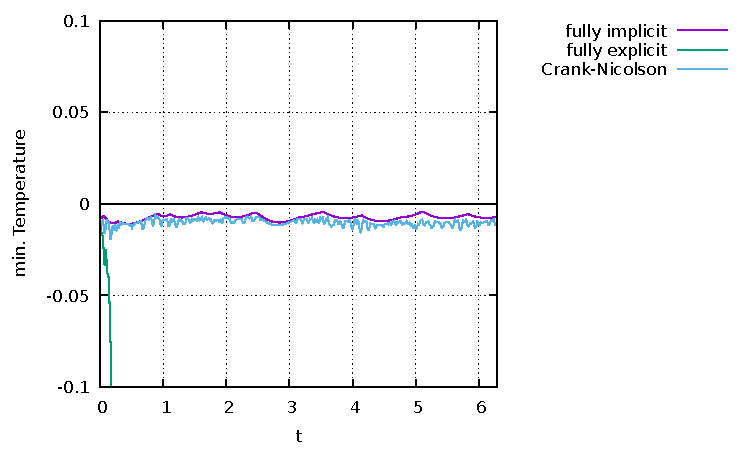
\includegraphics[width=5.7cm]{python_codes/fieldstone_43/results/experiment1/Tmin.pdf}
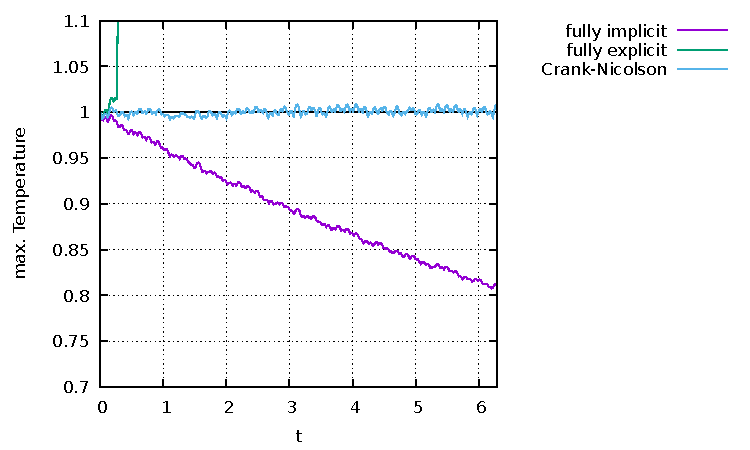
\includegraphics[width=5.7cm]{python_codes/fieldstone_43/results/experiment1/Tmax.pdf}
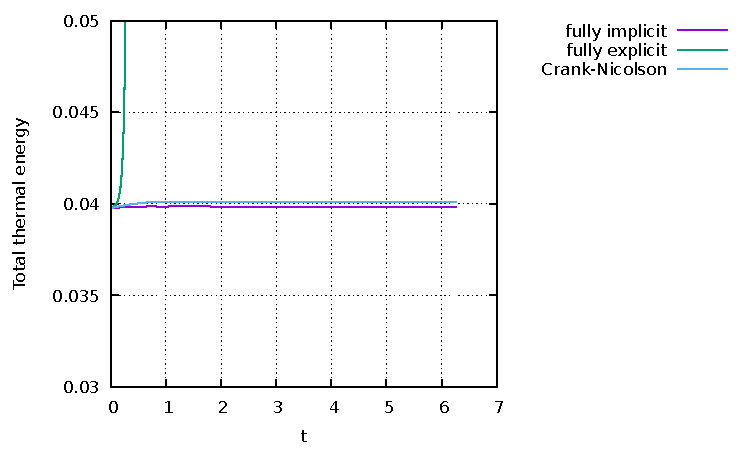
\includegraphics[width=5.7cm]{python_codes/fieldstone_43/results/experiment1/ET.pdf}\\
{\captionfont Time evolution of the min and max temperature and the total energy}
\end{center}
The conclusions are clear: the explicit method diverges quickly and is unusable. 
The fully implicit and Crank-Nicolson 
method yield similar energy conservation but the fully-implicit showcases 
a clear decrease in maximum temperature.


%...................................................................................
\subsubsection*{Effect of time step value} 
We can run the experiment (still a $2\pi$ rotation) 
with three different time steps ($\delta t=2\pi/30,2\pi/60,2\pi/120$) 
and we recover very similar results to those presented in \textcite{dohu03}:
\begin{center}
\includegraphics[height=8cm]{python_codes/fieldstone_43/results/experiment1/dohu03}
\includegraphics[height=8cm]{python_codes/fieldstone_43/results/experiment1/temps_30_60_120}\\
{\captionfont From top to bottom: $\delta t=2\pi/120,2\pi/60,2\pi/30$ with Crank-Nicolson. 
Left panel is taken from donea \& Huerta \cite{dohu03}. Results obtained with linear elements.}
\end{center}



%...................................................................
\subsubsection*{On the use of BDF methods} I have also implemented 
BDF1,2,3,4,5  (see Section~\ref{MMM-ss:hte_fem}). 
BDF2 outperforms BDF1 and is comparable to Crank-Nicolson. 
For reasons unknown to me, the BDF3 diverges after 100 time steps. So do 
BDF4 and BDF5 after even less timesteps. In the following picture the temperature is shown for 
BDF1,2,3 and Crank-Nicolson after a full rotation.

\begin{center}
\includegraphics[width=15cm]{python_codes/fieldstone_43/results/experiment1/Tbdf123crni.png}\\
{\captionfont Left to right: BDF1 (i.e. implicit euler), BDF2, BDF3, Crank-Nicolson}
\end{center}



%.....................................
\subsubsection*{On the effect of SUPG} 
I now turn to another aspect of this problem: what is the effect of the SUPG stabilisation 
scheme on the solution? In what follows Crank-Nicolson is used. 

\begin{center}
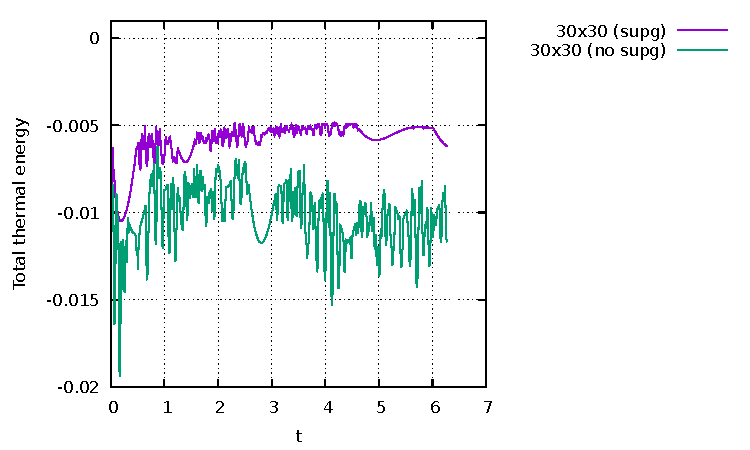
\includegraphics[width=7cm]{python_codes/fieldstone_43/results/experiment1/Tmin_supg}
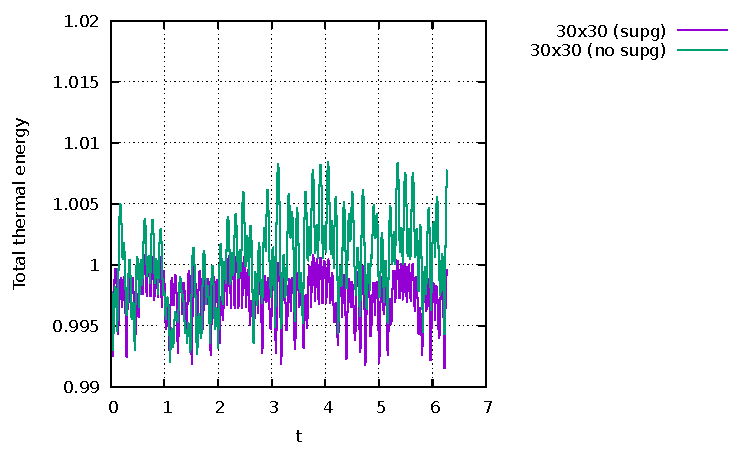
\includegraphics[width=7cm]{python_codes/fieldstone_43/results/experiment1/Tmax_supg}\\
{\captionfont Time evolution of min/max temperature with and without SUPG.} 
\end{center}

We find that SUPG yields a solution which min/max values are closer to the analytical ones.

\begin{center}
a)\includegraphics[width=4.8cm]{python_codes/fieldstone_43/results/experiment1/supg/solution_0000.pdf}
b)\includegraphics[width=4.8cm]{python_codes/fieldstone_43/results/experiment1/supg/solution_0100.pdf}
c)\includegraphics[width=4.8cm]{python_codes/fieldstone_43/results/experiment1/supg/solution_0200.pdf}
d)\includegraphics[width=4.8cm]{python_codes/fieldstone_43/results/experiment1/supg/solution_0300.pdf}
e)\includegraphics[width=4.8cm]{python_codes/fieldstone_43/results/experiment1/supg/solution_0400.pdf}
f)\includegraphics[width=4.8cm]{python_codes/fieldstone_43/results/experiment1/supg/solution_0500.pdf}\\
{\captionfont a,b,c,d,e,f) Temperature field throughout the $2\pi$ rotation.} 
\end{center}



%------------------------------------------------------------------------------
%------------------------------------------------------------------------------
%------------------------------------------------------------------------------
\newpage
\subsection*{Experiment 2 - Three objects rotation}

This setup is inspired by the one in the ASPECT 
manual\footnote{\url{https://aspect-documentation.readthedocs.io/en/latest/user/benchmarks/benchmarks/advection/doc/advection.html}}. The cone of the previous 
experiment is now replaced by three 'objects': a Zalesak disk \cite{zale79}, 
a sharp cone and a truncated cosine hill:

\begin{lstlisting}
for i in range(0,NV):
    xi=x[i]
    yi=y[i]
    if np.sqrt(xi**2+(yi-0.5)**2)<0.3 and (np.abs(xi)>=0.05 or yi>=0.7):
       T[i]=1
    if np.sqrt((x[i])**2+(y[i]+0.5)**2)<0.3:
       T[i]=1-np.sqrt((x[i])**2+(y[i]+0.5)**2)/0.3
    if np.sqrt((x[i]+0.5)**2+(y[i])**2)<0.3:
       T[i]=0.25*(1+np.cos(np.pi*np.sqrt((xi+0.5)**2+yi**2)/0.3))
\end{lstlisting}

The domain is $2\times2$, centered on the origin. The velocity is $\vec\upnu=(-y,x)$. Temperature 
is set to zero on all four sides (only on influx subsets). For this experiment the CFL number is set to 0.5
and the resolution is $64\times 64$ elements.

\begin{center}
\includegraphics[width=8cm]{python_codes/fieldstone_43/results/experiment2/buildings}
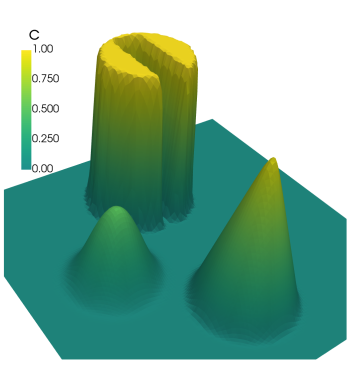
\includegraphics[width=5.2cm]{python_codes/fieldstone_43/results/experiment2/kome22}\\
{\captionfont Left: ASPECT manual; Right: taken from \textcite{kome22} (2022).}
\end{center}


\begin{center}
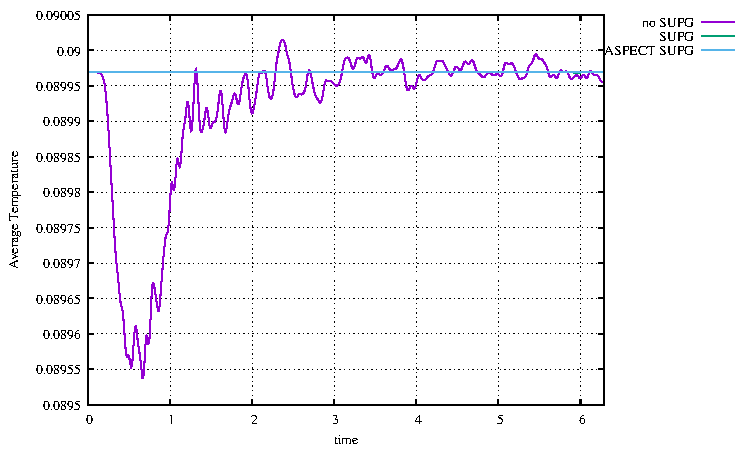
\includegraphics[width=8cm]{python_codes/fieldstone_43/results/experiment2/avrg_T}
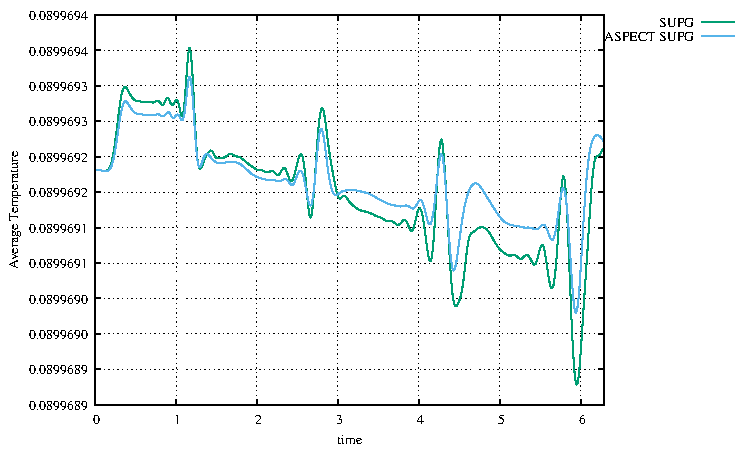
\includegraphics[width=8cm]{python_codes/fieldstone_43/results/experiment2/avrg_T2}\\
{\captionfont Averave temperature in the domain as a function of time. 
Left: all three cases. Right: only SUPG cases.}
\end{center}

\begin{center}
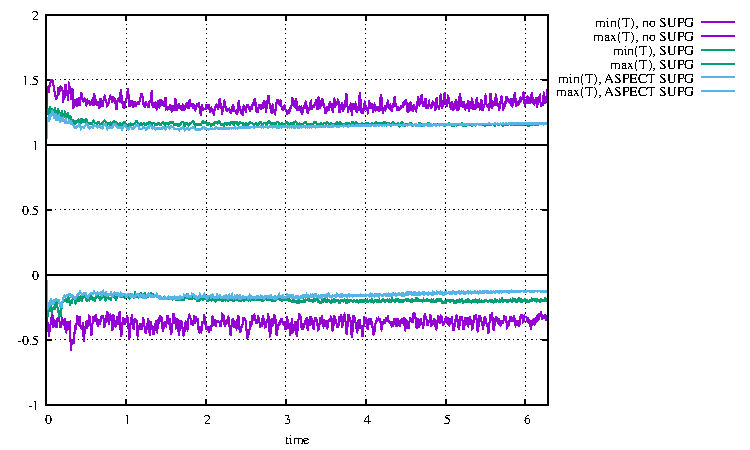
\includegraphics[width=8cm]{python_codes/fieldstone_43/results/experiment2/stats_T}
\end{center}

\begin{center}
\includegraphics[width=3.72cm]{python_codes/fieldstone_43/results/experiment2/supg/solution_0000.pdf}
\includegraphics[width=3.72cm]{python_codes/fieldstone_43/results/experiment2/supg/solution_0200.pdf}
\includegraphics[width=3.72cm]{python_codes/fieldstone_43/results/experiment2/supg/solution_0400.pdf}
\includegraphics[width=3.72cm]{python_codes/fieldstone_43/results/experiment2/supg/solution_0600.pdf}\\
\includegraphics[width=3.72cm]{python_codes/fieldstone_43/results/experiment2/supg/solution_0800.pdf}
\includegraphics[width=3.72cm]{python_codes/fieldstone_43/results/experiment2/supg/solution_1000.pdf}
\includegraphics[width=3.72cm]{python_codes/fieldstone_43/results/experiment2/supg/solution_1130.pdf}\\
{\captionfont Time evolution of the temperature field with Crank-Nicolson, with SUPG.}
\end{center}


\begin{center}
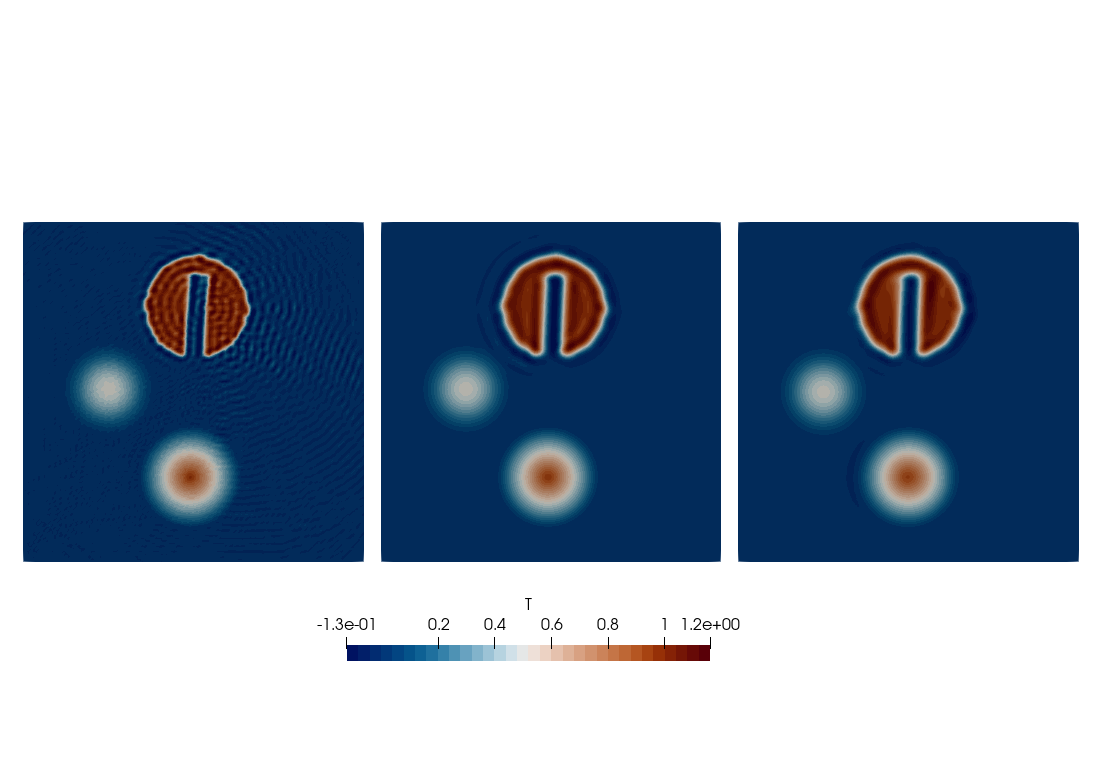
\includegraphics[width=15cm]{python_codes/fieldstone_43/results/experiment2/Temps}\\
{\captionfont Left: no SUPG; middle: with SUPG; right: ASPECT with SUPG}
\end{center}


%------------------------------------------------------------------------------
\newpage
\subsection*{Experiment 3 - 1D step advection}

This experiment comes from Appendix A of Thieulot (2011) \cite{thie11}.
The unit segment is discretised by means of 64 elements, 
over which a unit velocity field is prescribed.
The discontinuity is initially
placed at $x=1/4$ and after a time $t=0.5$, it is expected to have
reached the position $x=3/4$.
Temperature boundary conditions are $T=1$ on the left. 
Note that the simulation is actually carried out in 2D with a $1\times0.25$ domain 
discretised by means of $64\times16$ elements.
CFL number is set to 0.25.

%\[
%\tau_{supg} = \frac{h}{2 d |\vec{\upnu}|} = \frac{\sqrt{2}/50}{2 \cdot 1 \cdot 1} = 0.01414
%\]

%\begin{center}
%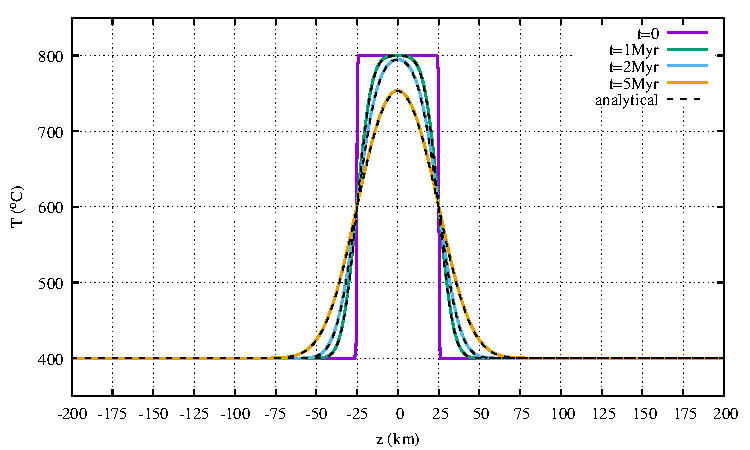
\includegraphics[width=8cm]{python_codes/fieldstone_43/results/experiment3/Q1/supg1/T.pdf}
%\includegraphics[width=6cm]{python_codes/fieldstone_43/results/experiment3/Q1/supg1/solution_0250.pdf}
%\end{center}


\[
\tau_{supg} = \frac{h}{2 d |\vec{\upnu}|} = \frac{\sqrt{2}/64}{2 \cdot 2 \cdot 1} = 0.005524
\]

\begin{center}
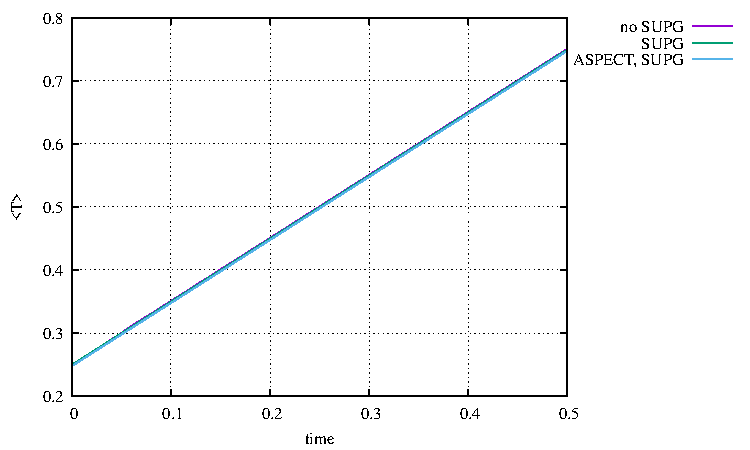
\includegraphics[width=5.7cm]{python_codes/fieldstone_43/results/experiment3/Q2/avrg_T.pdf}
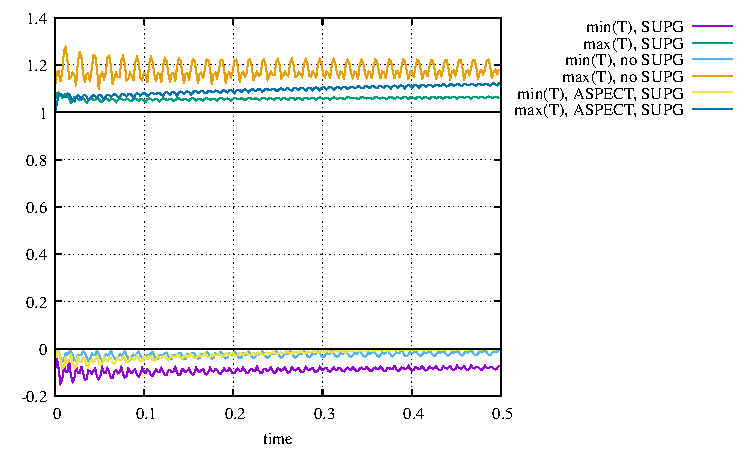
\includegraphics[width=5.7cm]{python_codes/fieldstone_43/results/experiment3/Q2/stats_T.pdf}
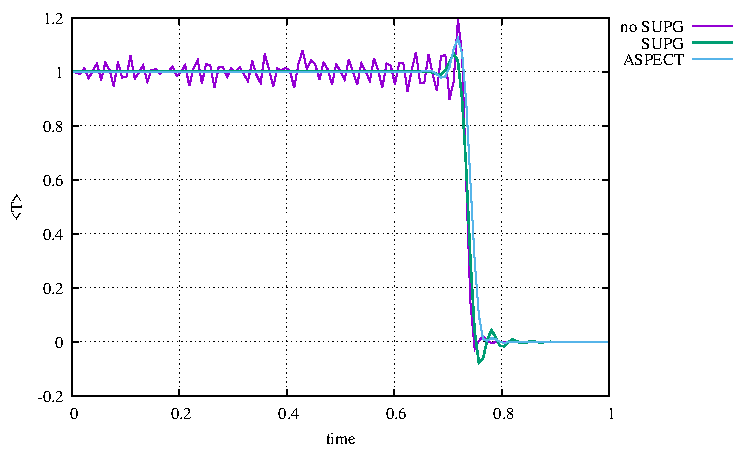
\includegraphics[width=5.7cm]{python_codes/fieldstone_43/results/experiment3/Q2/temperature.pdf}
\end{center}


\begin{center}
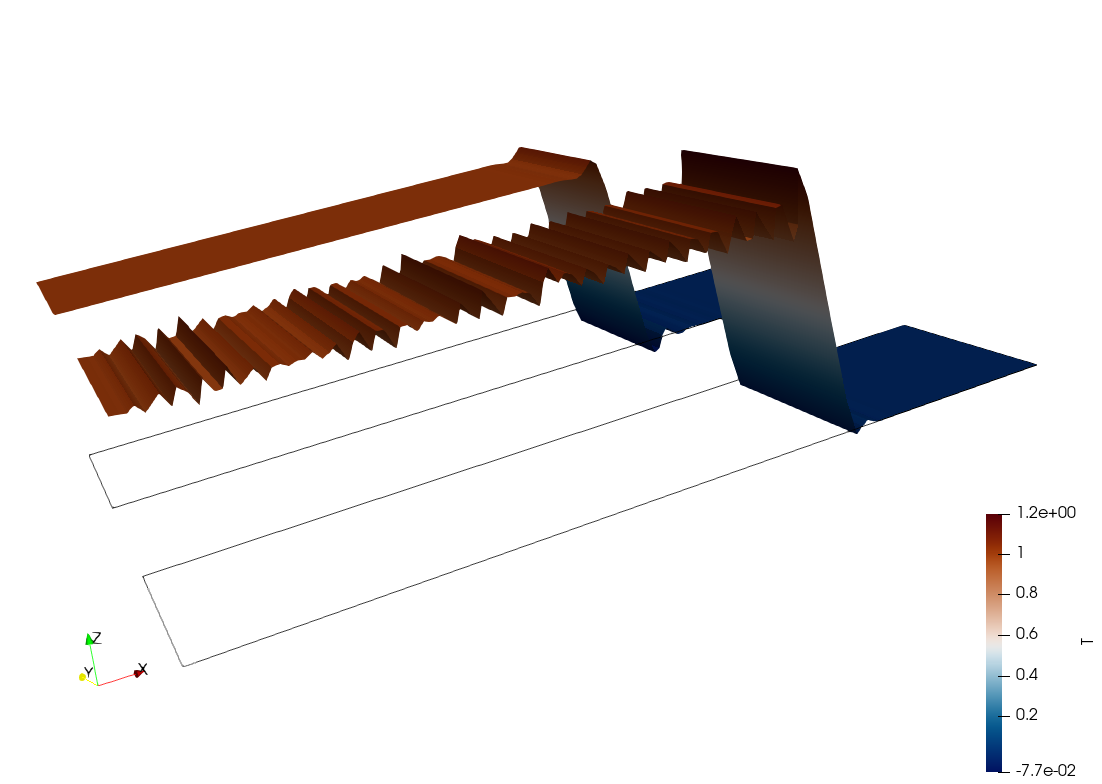
\includegraphics[width=10cm]{python_codes/fieldstone_43/results/experiment3/Q2/compT}\\
{\captionfont Temperature field at the end of the simulation. No SUPG in the front, 
with SUPG in the back.}
\end{center}






%...........................................................................................
\newpage
\subsection*{Experiment 4 - Steady state sideways 2D advection}

This experiment is somewhat similar to the one in \stone~65.
The domain is a unit square, and the velocity is given 
by $\vec\upnu=(\cos \theta, \sin\theta)$ with $\theta=\pi/6$.
The temperature is prescribed on the left side only, i.e. $T=1$ for $x=0$, $y=[0,1]$ 
(corners included), and 
on the bottom (left corner excluded) with $T=0$. The other two sides 
are left free. Initial temperature is $T=0$.
The resolution is $10\times10$ and the CFL number is set to $C_{\tt CFL}=0.1$. 
The model is run up to $t=3$ (steady state is then reached). 

\begin{center}
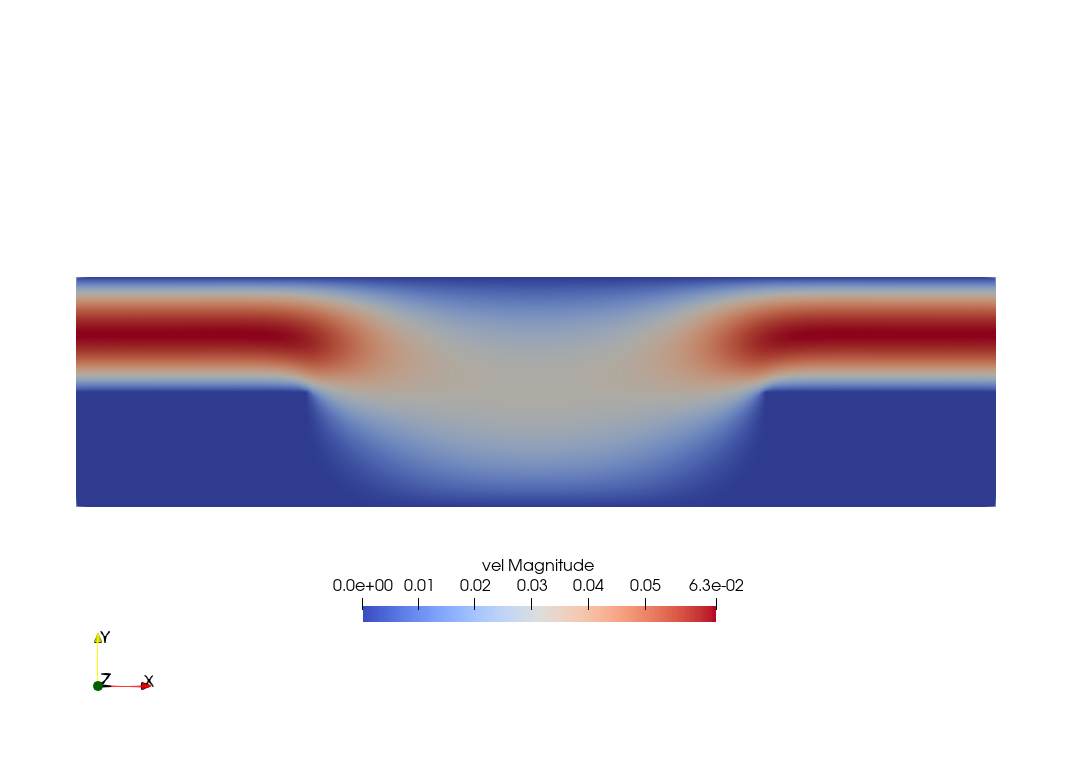
\includegraphics[width=5.6cm]{python_codes/fieldstone_43/results/experiment4/vel}
\includegraphics[width=5.6cm]{python_codes/fieldstone_43/results/experiment4/Tss}
\includegraphics[width=5.6cm]{python_codes/fieldstone_43/results/experiment4/Tss3D}\\
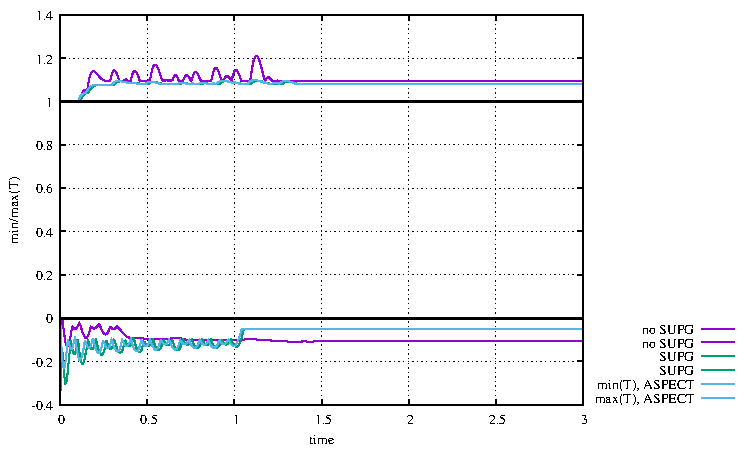
\includegraphics[width=8cm]{python_codes/fieldstone_43/results/experiment4/stats_T}
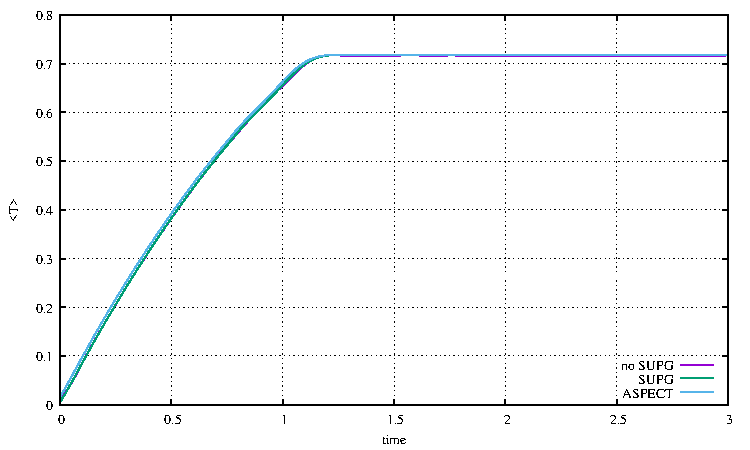
\includegraphics[width=8cm]{python_codes/fieldstone_43/results/experiment4/avrg_T}
\end{center}

%...........................................................................................
\newpage
\subsection*{Experiment 5 - Steady state rotation }

The domain is a unit square. The velocity field is given by $\vec\upnu=(y,1-x)$. 
The initial temperature is $T(x,y)=0$. 
Influx boundary conditions are prescribed on the left and bottom boundaries so
$T=0$ is prescribed on the left while at the bottom $T=0$ is prescribed if $x<1/3$ and $T=1$
otherwise. Resolution is $16\times16$ and the CFL number is set to $C_{CFL}=0.25$. 
The model is run up to $t=4$ (steady state is then reached).

\begin{center}
\includegraphics[height=4.cm]{python_codes/fieldstone_43/results/experiment5/vel}
\includegraphics[height=4.cm]{python_codes/fieldstone_43/results/experiment5/T}
\includegraphics[height=4.cm]{python_codes/fieldstone_43/results/experiment5/T3D}\\
{\captionfont Left: no SUPG, Right: SUPG.}
\end{center}


\begin{center}
\includegraphics[width=7cm]{python_codes/fieldstone_43/results/experiment5/stats_T}
\includegraphics[width=7cm]{python_codes/fieldstone_43/results/experiment5/avrg_T}
\end{center}

Note that it is currently not possible to run this experiment with ASPECT (?).

%...........................................................................................
\newpage
\subsection*{Experiment 6 - Bending beam}

The domain is a Cartesian box of size $1000\times1000$km, 
discretised with $50\times50$ elements. The CFL number is set to 0.25.
The top boundary is an inflow while the bottom boundary is an outflow.
We then prescribe $T=0$ at the top. On the left side $T=1$ if prescribed if $200<y<800$km 
and 0 elsewhere.
The initial temperature field is a $800\times600$km square attached to the left (see figure).
The velocity is given by $\vec{\upnu}=(0,-x/Lx\cdot v_0)$  with $v_0=1~\si{\cm\per\year}$:

\begin{center}
\includegraphics[width=7cm]{python_codes/fieldstone_43/results/experiment6/setup}
\end{center}

Note that in this case, because of the very small velocity and the large size of the elements,  
the reported $\tau$ value is about $10^{13-15}$.

\begin{center}
\includegraphics[width=14cm]{python_codes/fieldstone_43/results/experiment6/T}\\
{\captionfont Left: no SUPG; right: with SUPG}
\end{center}

Although SUPG removes the small wiggles, it does unfortunately not get rid of the 
large scale under/overshoots. 

\begin{center}
\includegraphics[width=7cm]{python_codes/fieldstone_43/results/experiment6/stats_T}
\includegraphics[width=7cm]{python_codes/fieldstone_43/results/experiment6/avrg_T}
\end{center}

We can also plot the temperature on the vertical line given by $x=L_x/2$:
\begin{center}
\includegraphics[width=8cm]{python_codes/fieldstone_43/results/experiment6/diagonal}
\end{center}


%...........................................................................................
\newpage
\subsection*{Experiment 7 - Beam in a whirl}

The setup is identical to experiment 6 but the velocity is now 
given by the equations of Section~\ref{MMM-mms1} which have been multiplied by 100 cm/year 
to arrive at a max velocity in the domain of approximately 1cm/year.
Since the velocity is parallel/zero on all four boundaries we can prescribe the 
temperature on all four boundaries. The CFL number is set to 0.25.

\begin{center}
\includegraphics[width=7cm]{python_codes/fieldstone_43/results/experiment7/T}
\includegraphics[width=7cm]{python_codes/fieldstone_43/results/experiment7/vel}\\
{\captionfont Left: Initial temperature field in the domain. Right: velocity field.}
\end{center}

\begin{center}
\includegraphics[width=14cm]{python_codes/fieldstone_43/results/experiment7/T96}\\
{\captionfont Left: no SUPG; right: with SUPG. Resolution $96^2$.}
\end{center}

\begin{center}
\includegraphics[width=8cm]{python_codes/fieldstone_43/results/experiment7/stats_T}
\includegraphics[width=8cm]{python_codes/fieldstone_43/results/experiment7/avrg_T}\\
{\captionfont Temperature statistics (min,max,avrg) as a function of time 
for various resolutions with and without SUPG.}
\end{center}

We can also look at a transect of the temperature field from the upper-left corner
down to the lower-right corner:

\begin{center}
\includegraphics[width=8cm]{python_codes/fieldstone_43/results/experiment7/diagonal}
\includegraphics[width=8cm]{python_codes/fieldstone_43/results/experiment7/diagonal_supg}
\end{center}
With SUPG the ripples are mostly gone, but over/undershoots near large gradients 
are about the same with and without supg.

(note that the results above were obtained with slightly different b.c.)

%...........................................................................................
\newpage
\subsection*{Experiment 8 - 1D Cosine hill advection}

The setup originates in Li \cite[ex 5.2]{li06}.
The domain has dimension $L_x=1$. 
The temperature is prescribed on the left to be zero (the right boundary is an outflux
no no temperature can be prescribed there).
The initial temperature is given by
\[
T(x,0)=
\left\{
\begin{array}{ll}
\sin (10 \pi x) & \textrm{for } x< 0.1 \\
0               & \textrm{for } x\geq 0.1 
\end{array}
\right.
\]
The velocity is set to $u=0.1$.
We use a mesh of $200\times 4$ elements and a CFL number of 0.5. 
We run the model to time $t=8$.

\begin{center}
\includegraphics[width=4cm]{python_codes/fieldstone_43/results/experiment8/Temp0000}
\includegraphics[width=4cm]{python_codes/fieldstone_43/results/experiment8/Temp0050}
\includegraphics[width=4cm]{python_codes/fieldstone_43/results/experiment8/Temp0100}
\includegraphics[width=4cm]{python_codes/fieldstone_43/results/experiment8/Temp0150}\\
\includegraphics[width=4cm]{python_codes/fieldstone_43/results/experiment8/Temp0200}
\includegraphics[width=4cm]{python_codes/fieldstone_43/results/experiment8/Temp0250}
\includegraphics[width=4cm]{python_codes/fieldstone_43/results/experiment8/Temp0300}
\end{center}

\begin{center}
\includegraphics[width=8cm]{python_codes/fieldstone_43/results/experiment8/stats_T.pdf}
\includegraphics[width=8cm]{python_codes/fieldstone_43/results/experiment8/avrg_T.pdf}\\
\includegraphics[width=8cm]{python_codes/fieldstone_43/results/experiment8/diagonal}
\end{center}



\newpage
%...........................................................................................
\newpage
\subsection*{Experiment 9 - wiggles advection (deal.II step-9)}

The setup for this experiment is borrowed from step-9 of deal.II, found at 
\url{https://www.dealii.org/current/doxygen/deal.II/step_9.html}.
I have only changed the notations of the main variables to be consistent 
with the previous experiments of this \stone.

We wish to solve the steady-state advection equation 
$\vec\upnu \cdot \vec\nabla T = f$ 
where $\vec\upnu(\vec r)$ is  is a vector field that describes the advection direction and speed,
$f(\vec r)$ is a source function, and $T(\vec r)$ is the solution. 

At the inflow, the above equation needs to be augmented by boundary conditions: 
$T=g$ on $\partial\Omega_-$ where $\partial\Omega_-$ describes the inflow portion 
of the boundary and is formally defined by
\[
\partial\Omega_- = \left\{  \vec{r} \in \partial\Omega : \vec{\upnu}\cdot\vec{n} <0  \right\}
\]
and $\vec{n}$ being the outward normal to the domain. This definition is quite intuitive, 
since as $\vec{n}$ points outward, the scalar product with $\vec{\upnu}$ can only be negative if the transport direction $\vec{\upnu}$ points inward, i.e. at the inflow boundary. The mathematical theory states that we must not pose any boundary condition on the outflow part of the boundary.

Unfortunately, the equation stated above cannot be solved in a stable way using the standard finite element method. The problem is that solutions to this equation possess insufficient regularity perpendicular to the transport direction: while they are smooth along the streamlines defined by the ``wind field'' $\vec{\upnu}$, they may be discontinuous perpendicular to this direction.

We set $\Omega=[-1,1]^2$, with 
\begin{eqnarray}
\vec{\upnu} &=& \left(2, 1+\frac45\sin(8\pi x) \right) \nn\\
f&=&1/10s^2 \qquad \text{with} \quad s=0.1 \quad \text{for} \quad |\vec{r}-\vec{r}_0|<s \quad \text{otherwise}\; 0\nn\\ 
\vec{r}_0 &=& (-\frac34,-\frac34) \nn\\
g&=&\exp(5(1-|\vec{r}|^2))\sin(16\pi |\vec{r}|^2)
\end{eqnarray}

Finally a few additional comments are in order:
\begin{enumerate}
\item The advection field $\vec{\upnu}$ transports the solution roughly in diagonal direction 
from lower left to upper right, but with a wiggle structure superimposed; 
\begin{center}
\includegraphics[width=4cm]{python_codes/fieldstone_43/images/vel}
\end{center}

\item The right hand side adds to the field generated by the inflow boundary conditions a blob 
in the lower left corner, which is then transported along; 
\item The inflow boundary conditions impose a weighted sinusoidal structure that is transported along 
with the flow field. Since $|\vec{r}|\ge 1$ on the boundary, the weighting term never gets very large.
\end{enumerate}

\begin{center}
\includegraphics[width=8cm]{python_codes/fieldstone_43/images/step-9-grid-9.png}
\includegraphics[width=8cm]{python_codes/fieldstone_43/images/step-9-solution-9.png}\\
{\captionfont Taken from step-9 webpage. Grid and solution.}
\end{center}

The code implements time stepping so I am running models until steady state is reached. 
Given the velocity field and the size of the box, I found that $t_{final}=1.25$ is sufficient.
The initial temperature field is set to zero. The source term generates a hot spot in a circle 
in the lower left part of the domain while the boundary conditions imposed on the left and bottom 
boundaries generate a temperature field that is advected inward:

\begin{center}
\includegraphics[width=5.7cm]{python_codes/fieldstone_43/results/experiment9/T.0000.png}
\includegraphics[width=5.7cm]{python_codes/fieldstone_43/results/experiment9/T.0010.png}
\includegraphics[width=5.7cm]{python_codes/fieldstone_43/results/experiment9/T.0020.png}\\
\includegraphics[width=5.7cm]{python_codes/fieldstone_43/results/experiment9/T.0030.png}
\includegraphics[width=5.7cm]{python_codes/fieldstone_43/results/experiment9/T.0040.png}\\
{\captionfont Time evolution of the 
temperature field using $Q_2$ basis functions. 
Results obtained with $32\times 32$ grid for $C_{CFL}=0.5$ without SUPG.}
\end{center}


The following plots show the min/max values of the field and its average for three
different resolutions:
\begin{center}
\includegraphics[width=8cm]{python_codes/fieldstone_43/results/experiment9/stats_T.pdf}
\includegraphics[width=8cm]{python_codes/fieldstone_43/results/experiment9/avrg_T.pdf}\\
{\captionfont Results obtained with $Q_1$ and $Q_2$ basis functions for $C_{CFL}=0.5$ without SUPG.}
\end{center}

\begin{center}
\includegraphics[width=4cm]{python_codes/fieldstone_43/results/experiment9/T32.png}
\includegraphics[width=4cm]{python_codes/fieldstone_43/results/experiment9/T48.png}
\includegraphics[width=4cm]{python_codes/fieldstone_43/results/experiment9/T64.png}
\includegraphics[width=4cm]{python_codes/fieldstone_43/results/experiment9/T80.png}\\
{\captionfont Results obtained with $Q_2$ basis functions for $C_{CFL}=0.5$ without SUPG. 
From left to right: meshes are $32^2$, $48^2$, $64^2$ and $80^2$. Obviously this `Cold and Hot' 
colorscale is objectively a very bad one but it allows me to compare (visually) with the results obtained with
deal.II shown above.}
\end{center}

One can also plot the temperature field on a line roughly perpendicular to the 
direction of the velocity field, i.e. from the upper-left corner to 
the lower-right corner:
\begin{center}
\includegraphics[width=12cm]{python_codes/fieldstone_43/results/experiment9/diagonal.pdf}
\end{center}
We see that in order to capture the fine features of the temperature field 
much higher resolutions are needed which lead me to implement a steady state mode
that removes the $\partial_tT$ term and yields the desired steady state solution 
after only one solve. This proves to be necessary for resolutions higher than $64^2$.

\begin{center}
\includegraphics[width=12cm]{python_codes/fieldstone_43/results/experiment9/512_Q2/T.png}\\
{\captionfont Steady-state temperature field with $512^2$ mesh and $Q_2$ elements.}
\end{center}


We can now look at the effect of SUPG on these results. We therefore set $\tau=h/2|\vec\upnu|p$
where $p$ is the order of the $Q_p$ basis functions.

\begin{center}
\includegraphics[width=8cm]{python_codes/fieldstone_43/results/experiment9/stats_T_SUPG.pdf}
\includegraphics[width=8cm]{python_codes/fieldstone_43/results/experiment9/avrg_T_SUPG.pdf}\\
\includegraphics[width=12cm]{python_codes/fieldstone_43/results/experiment9/diagonal_SUPG.pdf}
\end{center}




